\section{图像重建}\label{sec:图像重建}
有了精心选好的图像样本后,我们需要把样本及其算出的辐射值
转化为用于显示或存储的像素值。根据信号处理理论,
我们需要做三件事来为输出图像中的每个像素计算最终值:
\begin{enumerate}
    \item 从图像样本集中重建连续的图像函数$\tilde{L}$.
    \item 对函数$\tilde{L}$预滤波以移除任何超过像素间隔对应的奈奎斯特上限的频率。
    \item 在像素位置采样$\tilde{L}$以计算最终像素值。
\end{enumerate}

因为我们知道我们将只在像素位置处重采样函数$\tilde{L}$,
所以没有必要构建该函数的显式表示。
相反,我们可以用单个滤波函数把前两步结合起来。

回想如果已经用大于奈奎斯特频率的频率对原始函数进行均匀采样
并用sinc滤波器重建,则第一步中的重建函数会完美匹配原始图像函数——
这是个壮举,毕竟我们只有样本点。
但因为图像函数几乎总是有比采样率所能处理的还高的频率(由边缘等造成),
我们选择对其不均匀地采样,把混叠换成噪声。

理想重建背后的理论依赖于均匀间隔的样本。
尽管已有大量将该理论拓展到非均匀采样的尝试,
但目前该问题还没有公认的解决方法。
此外,因为知道采样率不足以刻画函数,所以完美重建是不可能的。
采样理论领域最近的研究重新看待了重建问题,
明确承认实践中完美重建通常是不可能的。
这一观点的微小转变带来了强大的重建新技术。
例如参见\citet{843002}了解关于这些进展的调研。
特别地,重建理论的研究目标已经从完美重建转为
开发能被证明可最小化重建函数与原始函数间差异的重建技术,
\emph{而不管原始函数是否是带限的}。

尽管pbrt中用的重建技术不是直接建立在这些新方法上的,
但它们能解释实践者的经验,即对图像合成所取的样本应用
完美重建技术通常不会得到最高质量的图像。
\begin{figure}[htbp]
    \centering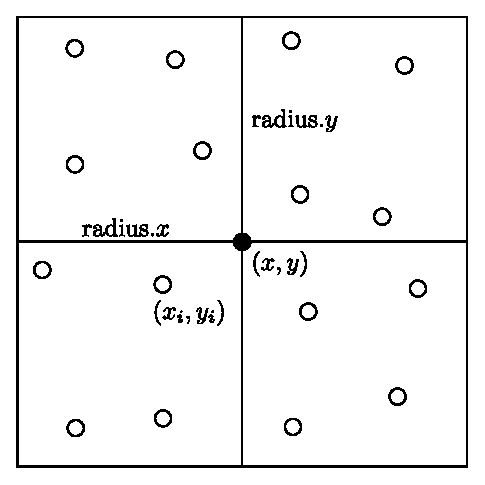
\includegraphics[width=0.5\linewidth]{chap07/2dimagefiltering.eps}
    \caption{2D图像滤波。为了给位于$(x,y)$处标为实心圆的像素
    计算滤波后的像素值,要考虑在$(x,y)$周围范围{\ttfamily radius.x}和
    {\ttfamily radius.y}以内方盒中的所有图像样本。
    每个表示为空心圆的图像样本$(x_i,y_i)$,都被2D滤波函数$f(x-x_i,y-y_i)$赋权。
    所有样本的加权平均即是最终的像素值。}
    \label{fig:7.38}
\end{figure}

为了重建像素值,我们将考虑在一特定像素旁对样本插值的问题。
为了给像素$I(x,y)$计算最终值,插值结果是计算加权平均
\begin{align}\label{eq:7.12}
    I(x,y)=\frac{\sum\limits_i {f(x-x_i,y-y_i)w(x_i,y_i)L(x_i,y_i)}}{\sum\limits_i {f(x-x_i,y-y_i)}}\, ,
\end{align}
其中
\begin{itemize}
    \item $L(x_i,y_i)$是位于$(x_i,y_i)$的第$i$个样本的辐亮度值;
    \item $w(x_i,y_i)$是\refvar{Camera}{}返回的样本贡献权重。
          如\refsub{相机测量方程}和\refsub{采样相机1}所述,
          计算这些权重的方法决定了胶片度量哪个辐射度学量;
    \item $f$是滤波函数。
\end{itemize}

\reffig{7.38}展示了位于$(x,y)$的像素,它有个在$x$和$y$方向
范围分别为{\ttfamily radius.x}和{\ttfamily radius.y}的像素滤波器。
在滤波器范围给出的方盒内的所有样本都可能对该像素值有贡献,
这取决于滤波函数值$f(x-x_i,y-y_i)$.

这里sinc滤波器不是合适的选择:回想当基本函数有超过奈奎斯特上限的频率时
理想sinc滤波器容易振铃(吉布斯现象),这意味着图像中的边缘在附近像素处
有微弱重复的边缘副本。此外,sinc滤波器有\emph{无限支撑}:
距离其中心的有限距离内它不会衰减到零,
所以对于每个输出像素都会需要滤波所有图像样本。实践中没有唯一最好的滤波函数。
为特定场景选择最好的需要结合定量评估与定性判断。

\subsection{滤波函数}\label{sub:滤波函数}
pbrt中的所有滤波器实现都从抽象类\refvar{Filter}{}派生,
它为滤波中用的函数$f(x,y)$提供了接口;见\refeq{7.12}。
(\refsec{胶片与成像管道}描述的)类\refvar{Film}{}存有指向\refvar{Filter}{}的指针
并在把图像样本的贡献累加到最终图像时对其滤波。
(\reffig{7.39}展示比较了用本节各种滤波器来重建像素值而渲染出的图像放大区域。)
基类\refvar{Filter}{}定义在文件\href{https://github.com/mmp/pbrt-v3/blob/master/src/core/filter.h}{\ttfamily core/filter.h}
和\href{https://github.com/mmp/pbrt-v3/blob/master/src/core/filter.cpp}{\ttfamily core/filter.cpp}中。
\begin{figure}[htbp]
    \centering
    \subfloat[矩形滤波器]{\includegraphics[width=0.65\linewidth]{chap07/crown-box.png}\label{fig:7.39.1}}\\
    \subfloat[高斯滤波器]{\includegraphics[width=0.65\linewidth]{chap07/crown-gaussian.png}\label{fig:7.39.2}}\\
    \subfloat[Mitchell-Netravali滤波器]{\includegraphics[width=0.65\linewidth]{chap07/crown-mitchell.png}\label{fig:7.39.3}}\\
    \caption{用来将图像样本转化为像素值的像素重建滤波器对最终图像的质量有明显的影响。
        这里我们看到用(a)矩形滤波器、(b)高斯以及(c) Mitchell-Netravali滤波器滤波的皇冠模型放大区域。
        注意Mitchell滤波器给出了最清晰的图像,而高斯则模糊了它。
        矩形是最不可取的,因为它允许高频混叠泄漏到最终图像中
        (例如注意沿明亮金色边缘的阶梯状模式)。}
    \label{fig:7.39}
\end{figure}

\begin{lstlisting}
`\initcode{Filter Declarations}{=}`
class `\initvar{Filter}{}` {
public:
    `\refcode{Filter Interface}{}`
    `\refcode{Filter Public Data}{}`
};
\end{lstlisting}

\begin{figure}[htbp]
    \centering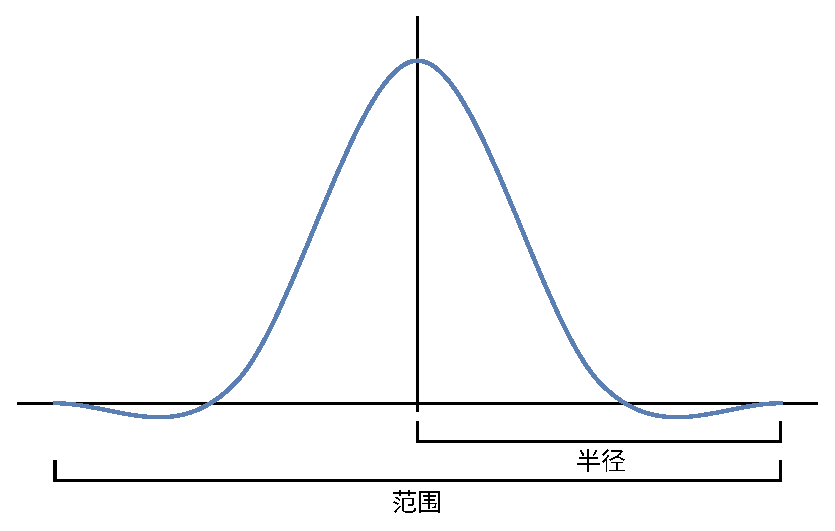
\includegraphics[width=0.6\linewidth]{chap07/filter-extent-radius.eps}
    \caption{pbrt中滤波器的范围是依据从原点到其截断点的半径来指定的。
        滤波器的支撑域是其整个非零范围,这里等于其半径的两倍。}
    \label{fig:7.40}
\end{figure}

所有滤波器中心都在原点$(0,0)$且定义了半径,超出半径时它们都取值为0;
该宽度也许在$x$和$y$方向是不同的。
构造函数接收半径值并和其倒数一块儿保存,以供滤波器实现使用。
滤波器在每个方向的整个范围(它的支撑域)是其相应半径值的两倍(\reffig{7.40})。
\begin{lstlisting}
`\initcode{Filter Interface}{=}\initnext{FilterInterface}`
`\refvar{Filter}{}`(const `\refvar{Vector2f}{}` &radius)
    : `\refvar[Filter::radius]{radius}{}`(radius),
      `\refvar[Filter::invRadius]{invRadius}{}`(`\refvar{Vector2f}{}`(1 / radius.x, 1 / radius.y)) { }
\end{lstlisting}
\begin{lstlisting}
`\initcode{Filter Public Data}{=}`
const `\refvar{Vector2f}{}` `\initvar[Filter::radius]{radius}{}`, `\initvar[Filter::invRadius]{invRadius}{}`;
\end{lstlisting}

\refvar{Filter}{}实现需要提供的唯一方法是\refvar[Filter::Evaluate]{Evaluate}{()}。
它接收一个给出了样本点相对于滤波器中心位置的2D点参数。
返回滤波器在该点的值。系统中别处的代码永远不会用滤波器范围外的点来调用滤波函数,
所以滤波器实现不需要检查这种情况。
\begin{lstlisting}
`\refcode{Filter Interface}{+=}\lastcode{FilterInterface}`
virtual `\refvar{Float}{}` `\initvar[Filter::Evaluate]{Evaluate}{}`(const `\refvar{Point2f}{}` &p) const = 0;
\end{lstlisting}

\subsubsection*{矩形滤波器}
图形学中最常用的滤波器之一是\keyindex{矩形滤波器}{box filter}{filter滤波器}
(且实际上当没有明确解决滤波和重建时,矩形滤波器就是\emph{事实上}的结果)。
矩形滤波器对图像的一个方形区域内的所有样本等值赋权。
尽管计算很高效,但它可能是最差的滤波器。
从\refsub{理想采样与重建}的讨论中回想矩形滤波器允许高频样本数据
泄漏到重建的值中。这会造成后混叠——
即使原始样本值足够高频以避免混叠,糟糕的滤波还是会引入误差。

\reffig{7.41}(a)展示了矩形滤波器的图像,
\reffig{7.42}展示了用矩形滤波器重建两个1D函数的结果。

对于之前我们用来说明吉布斯现象的阶跃函数,矩形滤波器尚能做得很好。
然而对于频率沿$x$轴增加的正弦函数结果则差得多。
不仅在低频时矩形滤波器把函数重建得很差,即使原始函数是光滑的也给出不连续的结果,
而且它在函数频率接近和超过奈奎斯特上限时也重建得很差。
\begin{lstlisting}
`\initcode{BoxFilter Declarations}{=}`
class `\initvar{BoxFilter}{}` : public `\refvar{Filter}{}` {
public:
    `\refvar{BoxFilter}{}`(const `\refvar{Vector2f}{}` &radius) : `\refvar{Filter}{}`(radius) { }
    `\refvar{Float}{}` `\refvar[BoxFilter::Evaluate]{Evaluate}{}`(const `\refvar{Point2f}{}` &p) const;
};
\end{lstlisting}

\begin{figure}[htbp]
    \centering
    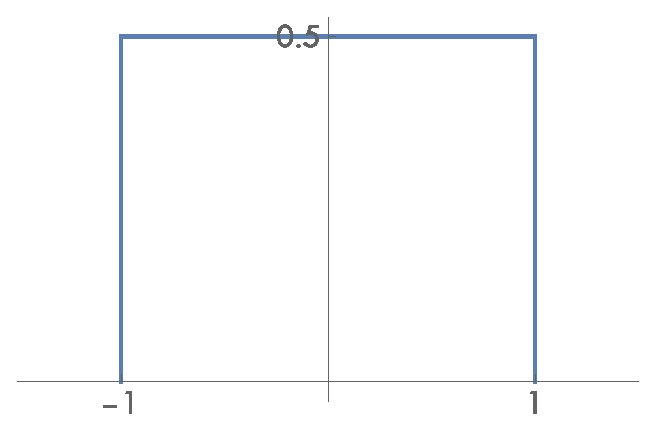
\includegraphics[width=0.45\linewidth]{chap07/box-filter.eps}\,
    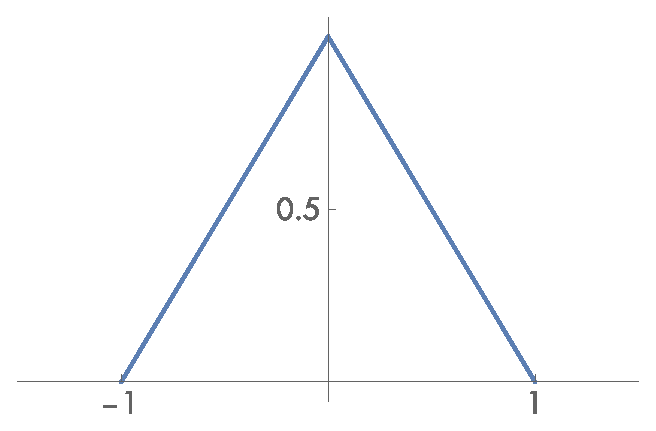
\includegraphics[width=0.45\linewidth]{chap07/triangle-filter.eps}
    \caption{(a)矩形滤波器和(b)三角滤波器的图示。尽管两者都不是特别好的滤波器,
        但它们的计算都很高效,易于实现,且对于评估其他滤波器是很好的基准线。}
    \label{fig:7.41}
\end{figure}
\begin{figure}[htbp]
    \centering
    \subfloat[]{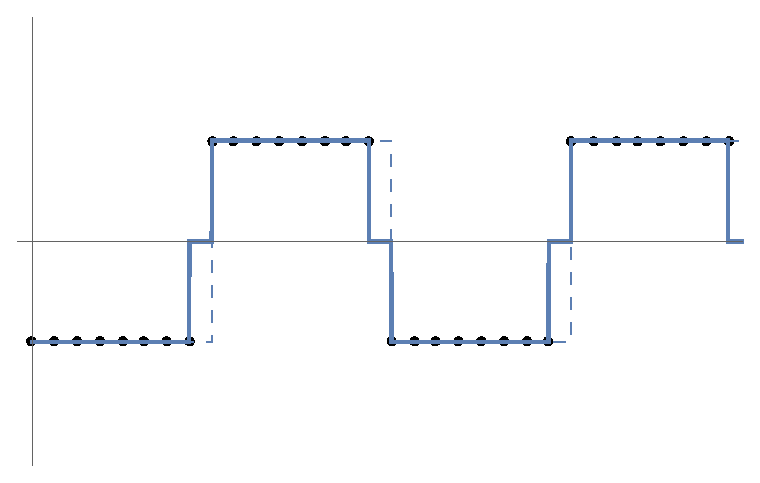
\includegraphics[width=0.49\linewidth]{chap07/box-recon-a.eps}\label{fig:7.42.1}}\,
    \subfloat[]{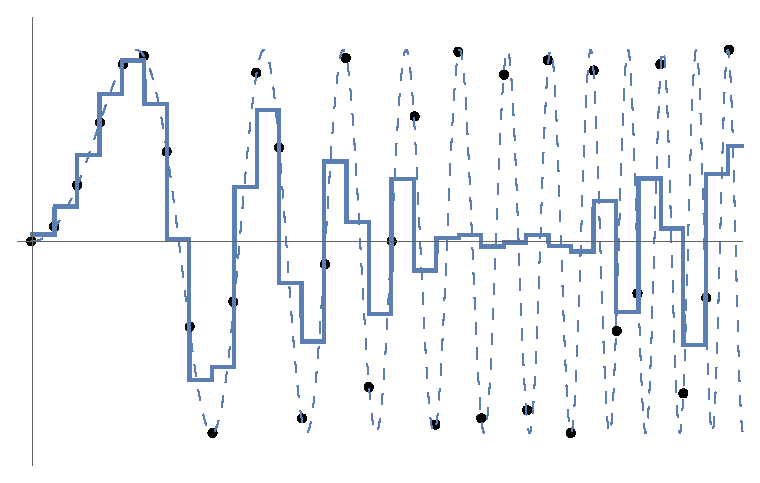
\includegraphics[width=0.49\linewidth]{chap07/box-recon-b.eps}\label{fig:7.42.2}}
    \caption{矩形滤波器重建(a)阶跃函数和(b)频率随着$x$增加而增加的正弦函数。
        该滤波器对阶跃函数如料想那样工作得很好,但对于正弦函数则工作得极其糟糕。}
    \label{fig:7.42}
\end{figure}

因为不会在$(x,y)$值超出滤波器范围时调用求值函数,
所以对于滤波函数值它可以总是返回1.
\begin{lstlisting}
`\initcode{BoxFilter Method Definitions}{=}`
`\refvar{Float}{}` `\refvar{BoxFilter}{}`::`\initvar[BoxFilter::Evaluate]{\refvar[Filter::Evaluate]{Evaluate}{}}{}`(const `\refvar{Point2f}{}` &p) const {
    return 1.;
}
\end{lstlisting}

\subsubsection*{三角滤波器}
\keyindex{三角滤波器}{triangle filter}{filter滤波器}给出了比矩形稍好的结果:在滤波器的方形范围上权重从滤波器中心起线性下降。
参见\reffig{7.41}(b)的三角滤波器图示。
\begin{lstlisting}
`\initcode{TriangleFilter Declarations}{=}`
class `\initvar{TriangleFilter}{}` : public `\refvar{Filter}{}` {
public:
    `\refvar{TriangleFilter}{}`(const `\refvar{Vector2f}{}` &radius) : `\refvar{Filter}{}`(radius) { }
    `\refvar{Float}{}` `\refvar[TriangleFilter::Evaluate]{Evaluate}{}`(const `\refvar{Point2f}{}` &p) const;
};
\end{lstlisting}

三角滤波器求值很简单:该实现只需计算同时基于滤波器在$x$和$y$方向上宽度的线性函数。
\begin{lstlisting}
`\initcode{TriangleFilter Method Definitions}{=}`
`\refvar{Float}{}` `\refvar{TriangleFilter}{}`::`\initvar[TriangleFilter::Evaluate]{\refvar[Filter::Evaluate]{Evaluate}{}}{}`(const `\refvar{Point2f}{}` &p) const {
    return std::max((`\refvar{Float}{}`)0, `\refvar[Filter::radius]{radius}{}`.x - std::abs(p.x)) *
           std::max((`\refvar{Float}{}`)0, `\refvar[Filter::radius]{radius}{}`.y - std::abs(p.y));
}
\end{lstlisting}

\subsubsection*{高斯滤波器}
不像矩形和三角滤波器那样,\keyindex{高斯滤波器}{Gaussian filter}{filter滤波器}在实践中给出了较好的结果。
该滤波器应用了中心在像素处且绕其径向对称的高斯凸块。
高斯从滤波器值中减去了它在范围末端的值,
好让滤波器在其界限处变为0(\reffig{7.43})。
比起其他一些滤波器,高斯确实倾向于造成最终图像轻微模糊,
但该模糊实际上能帮助遮住图像中留下的任何混叠。

\begin{figure}[htbp]
    \centering
    \subfloat[]{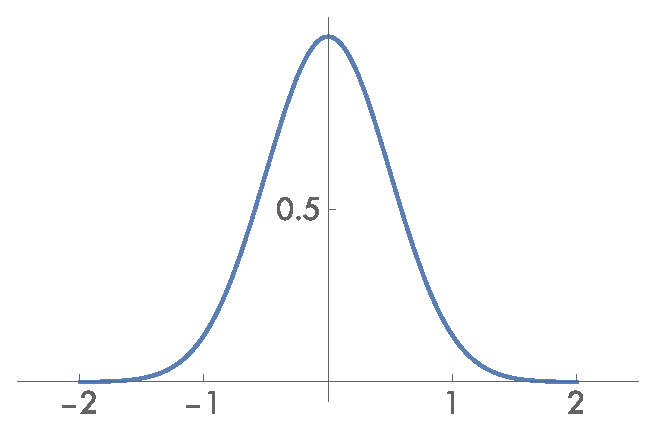
\includegraphics[width=0.49\linewidth]{chap07/gaussian-filter.eps}\label{fig:7.43.1}}\,
    \subfloat[]{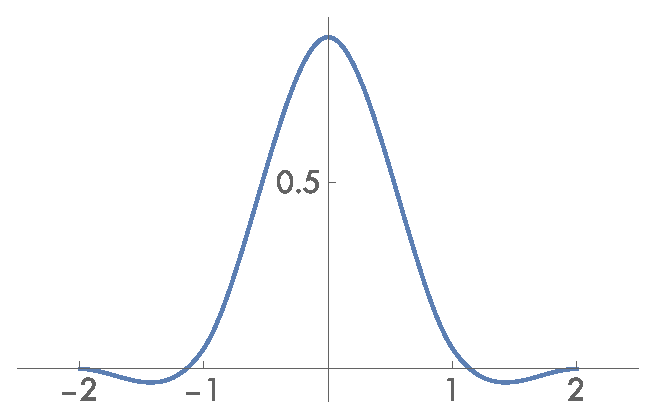
\includegraphics[width=0.49\linewidth]{chap07/mitchell-filter.eps}\label{fig:7.43.2}}
    \caption{(a)高斯滤波器和(b) $\displaystyle B=\frac{1}{3}$
        且$\displaystyle C=\frac{1}{3}$的Mitchell滤波器的图示,每个的宽度是2.
        高斯给出倾向于有点模糊的图像,而Mitchell滤波器的负波瓣有助于强调和
        锐化最终图像中的边界。}
    \label{fig:7.43}
\end{figure}

\begin{lstlisting}
`\initcode{GaussianFilter Declarations}{=}`
class `\initvar{GaussianFilter}{}` : public `\refvar{Filter}{}` {
public:
    `\refcode{GaussianFilter Public Methods}{}`
private:
    `\refcode{GaussianFilter Private Data}{}`
    `\refcode{GaussianFilter Utility Functions}{}`
};
\end{lstlisting}

半径为$r$的1D高斯滤波函数是
\begin{align*}
    f(x)={\mathrm{e}}^{-\alpha x^2}-{\mathrm{e}}^{-\alpha r^2}\, ,
\end{align*}
其中$\alpha$控制滤波器的衰减速率。更小的值使衰减更慢,给出更模糊的图像。
这里第二项保证高斯在其范围末端变为0而不是有个陡崖。
为了效率,构造函数在每个方向上预先计算了常数项${\mathrm{e}}^{-\alpha r^2}$.
\begin{lstlisting}
`\initcode{GaussianFilter Public Methods}{=}`
`\refvar{GaussianFilter}{}`(const `\refvar{Vector2f}{}` &radius, `\refvar{Float}{}` alpha)
    : `\refvar{Filter}{}`(radius), `\refvar[GaussianFilter::alpha]{alpha}{}`(alpha),
      `\refvar{expX}{}`(std::exp(-alpha * radius.x * radius.x)),
      `\refvar{expY}{}`(std::exp(-alpha * radius.y * radius.y)) { }
\end{lstlisting}
\begin{lstlisting}
`\initcode{GaussianFilter Private Data}{=}`
const `\refvar{Float}{}` `\initvar[GaussianFilter::alpha]{alpha}{}`;
const `\refvar{Float}{}` `\initvar{expX}{}`, `\initvar{expY}{}`;
\end{lstlisting}

因为2D高斯函数可分解为两个1D高斯的乘积,
所以实现调用函数\refvar{Gaussian}{()}
两次并把结果相乘。
\begin{lstlisting}
`\initcode{GaussianFilter Method Definitions}{=}`
`\refvar{Float}{}` `\refvar{GaussianFilter}{}`::`\initvar[GaussianFilter::Evaluate]{\refvar[Filter::Evaluate]{Evaluate}{}}{}`(const `\refvar{Point2f}{}` &p) const {
    return `\refvar{Gaussian}{}`(p.x, `\refvar{expX}{}`) * `\refvar{Gaussian}{}`(p.y, `\refvar{expY}{}`);
}
\end{lstlisting}
\begin{lstlisting}
`\initcode{GaussianFilter Utility Functions}{=}`
`\refvar{Float}{}` `\initvar{Gaussian}{}`(`\refvar{Float}{}` d, `\refvar{Float}{}` expv) const {
    return std::max((`\refvar{Float}{}`)0, `\refvar{Float}{}`(std::exp(-`\refvar[GaussianFilter::alpha]{alpha}{}` * d * d) - expv));
}
\end{lstlisting}

\subsubsection*{Mitchell滤波器}
设计滤波器是出了名的难,混合了数学分析与感知实验。
\citet{10.1145/54852.378514}为了能以系统的方式
探索该空间而开发了一系列参数化滤波函数。
在分析了受试者对用各种参数值滤波后的图像的主观反应后,
它们开发的滤波器能很好地权衡\emph{振铃}(图像中的幻影边缘挨着实际边缘)
与\emph{模糊}(过于模糊的结果)——两种来自糟糕重建滤波器的常见伪影。

从\reffig{7.43.2}中注意到该滤波函数在其边缘处取负值;
它有\keyindex{负波瓣}{negative lobe}{}。
实践中这些负区域提升了边缘的清晰度,给出更保真的
\sidenote{译者注:原文crisper。}图像(降低模糊)。
然而如果它们变得太大,则振铃就开始进入图像。
此外,因为最终像素值可能因此变为负数,
所以最终需要将它们截断到合法输出范围。

\reffig{7.44}展示了该滤波器重建的两个测试函数。
它对于两者都做得非常好:对于阶跃函数有最小的振铃,
对于正弦函数也做得非常好,直到采样率不足以刻画函数细节。
\begin{figure}[htbp]
    \centering
    \subfloat[]{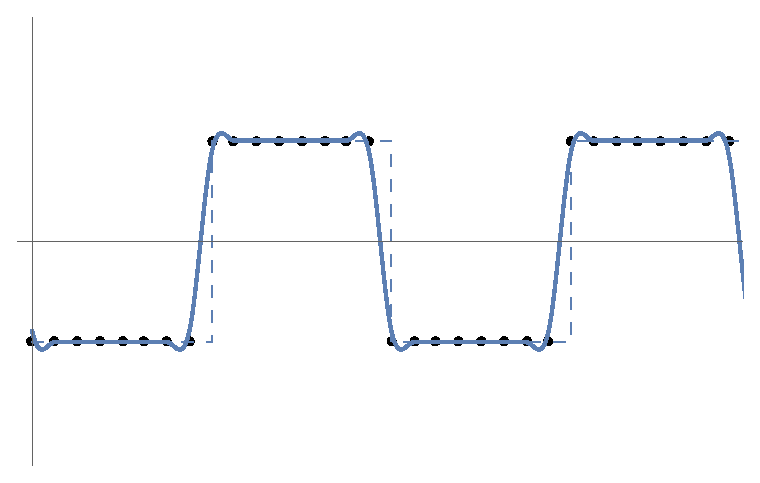
\includegraphics[width=0.49\linewidth]{chap07/mitchell-recon-a.eps}\label{fig:7.44.1}}\,
    \subfloat[]{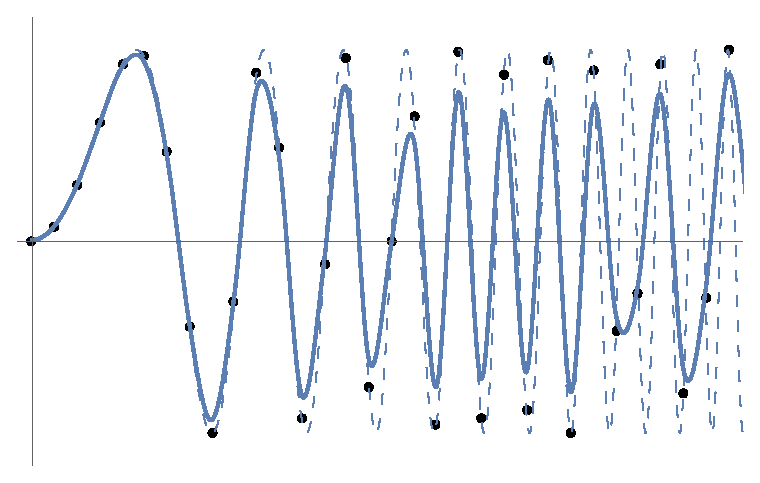
\includegraphics[width=0.49\linewidth]{chap07/mitchell-recon-b.eps}\label{fig:7.44.2}}
    \caption{Mitchell-Netravali滤波器用于重建示例函数。
        它对这两个函数都工作得很好,(a)对阶跃函数引入了最小振铃
        且(b)准确地表示了正弦曲线直到来自欠采样的混叠开始占主要地位。}
    \label{fig:7.44}
\end{figure}

\begin{lstlisting}
`\initcode{MitchellFilter Declarations}{=}`
class `\initvar{MitchellFilter}{}` : public `\refvar{Filter}{}` {
public:
    `\refcode{MitchellFilter Public Methods}{}`
private:
    const `\refvar{Float}{}` `\initvar[MitchellFilter::B]{B}{}`, `\initvar[MitchellFilter::C]{C}{}`;
};
\end{lstlisting}

Mitchell滤波器有两个参数叫$B$和$C$.
尽管这些参数可用任意值,但\citeauthor{10.1145/54852.378514}
建议它们位于直线$B+2C=1$上。
\begin{lstlisting}
`\initcode{MitchellFilter Public Methods}{=}\initnext{MitchellFilterPublicMethods}`
`\refvar{MitchellFilter}{}`(const `\refvar{Vector2f}{}` &radius, `\refvar{Float}{}` B, `\refvar{Float}{}` C)
    : `\refvar{Filter}{}`(radius), `\refvar[MitchellFilter::B]{B}{}`(B), `\refvar[MitchellFilter::C]{C}{}`(C) {
}
\end{lstlisting}

Mitchell-Netravali滤波器是在$x$和$y$方向上的1D滤波函数的乘积,
因此像高斯滤波器那样是可分离的(事实上pbrt中提供的所有滤波器都是可分离的)。
然而接口\refvar{Filter::Evaluate}{()}并不这样强制要求,
给将来实现新的滤波器提供更多灵活性。
\begin{lstlisting}
`\initcode{MitchellFilter Method Definitions}{=}`
`\refvar{Float}{}` `\refvar{MitchellFilter}{}`::`\initvar[MitchellFilter::Evaluate]{\refvar[Filter::Evaluate]{Evaluate}{}}{}`(const `\refvar{Point2f}{}` &p) const {
    return `\refvar{Mitchell1D}{}`(p.x * `\refvar[Filter::invRadius]{invRadius}{}`.x) * `\refvar{Mitchell1D}{}`(p.y * `\refvar[Filter::invRadius]{invRadius}{}`.y);
}
\end{lstlisting}

Mitchell滤波器中用的1D函数是个定义在范围$[-2,2]$上的偶函数。
通过联合定义在$[0,1]$上的三次多项式和另一个定义在$[1,2]$上的三次多项式得出了该函数。
这个结合的多项式还被平面$x=0$反射以得到完整的函数。
这些多项式由参数$B$和$C$控制,且被精心挑选以保证在$x=0$,$x=1$和$x=2$处
的$C^0$和$C^1$连续性。该多项式是
\begin{align*}
    f(x)=\frac{1}{6}\left\{
    \begin{array}{ll}
        (12-9B-6C)|x|^3+(-18+12B+6C)|x|^2+(6-2B),          & |x|<1\, ,      \\
        (-B-6C)|x|^3+(6B+30C)|x|^2+(-12B-48C)|x|+(8B+24C), & 1\le |x|<2\, , \\
        0,                                                 & \text{其他。}
    \end{array}
    \right.
\end{align*}

\begin{lstlisting}
`\refcode{MitchellFilter Public Methods}{+=}\lastcode{MitchellFilterPublicMethods}`
`\refvar{Float}{}` `\initvar{Mitchell1D}{}`(`\refvar{Float}{}` x) const {
    x = std::abs(2 * x);
    if (x > 1)
        return ((-`\refvar[MitchellFilter::B]{B}{}` - 6*`\refvar[MitchellFilter::C]{C}{}`) * x*x*x + (6*`\refvar[MitchellFilter::B]{B}{}` + 30*`\refvar[MitchellFilter::C]{C}{}`) * x*x +
                (-12*`\refvar[MitchellFilter::B]{B}{}` - 48*`\refvar[MitchellFilter::C]{C}{}`) * x + (8*`\refvar[MitchellFilter::B]{B}{}` + 24*`\refvar[MitchellFilter::C]{C}{}`)) * (1.f/6.f);
    else
        return ((12 - 9*`\refvar[MitchellFilter::B]{B}{}` - 6*`\refvar[MitchellFilter::C]{C}{}`) * x*x*x + 
                (-18 + 12*`\refvar[MitchellFilter::B]{B}{}` + 6*`\refvar[MitchellFilter::C]{C}{}`) * x*x +
                (6 - 2*`\refvar[MitchellFilter::B]{B}{}`)) * (1.f/6.f);
}
\end{lstlisting}

\subsubsection*{窗sinc滤波器}
最后,类\refvar{LanczosSincFilter}{}实现了基于sinc函数的滤波器。
实践中,sinc滤波器常常乘以另一个在一定距离后变为0的函数。
这得到了有限范围的滤波函数,它对具有合理性能的实现是必要的。
一个额外的参数$\tau$控制sinc函数在把值截断为0前要经过多少个周期
\sidenote{译者注:原文cycle,此处翻译为“周期”是折中做法,不是指严格意义上周期函数的周期。}。
\reffig{7.45}展示了三个周期的sinc函数图示,以及我们用的窗函数图示,
它由Lanczos开发。Lanczos窗就是sinc函数的中心波瓣,它被缩放以覆盖$\tau$个周期:
\begin{align*}
    w(x)=\frac{\sin\left(\displaystyle\frac{\pi x}{\tau}\right)}{\displaystyle\frac{\pi x}{\tau}}\, .
\end{align*}

\reffig{7.45}也展示了我们这里实现的滤波器,它是sinc函数和窗函数的乘积。
\begin{figure}[htbp]
    \centering
    \subfloat[]{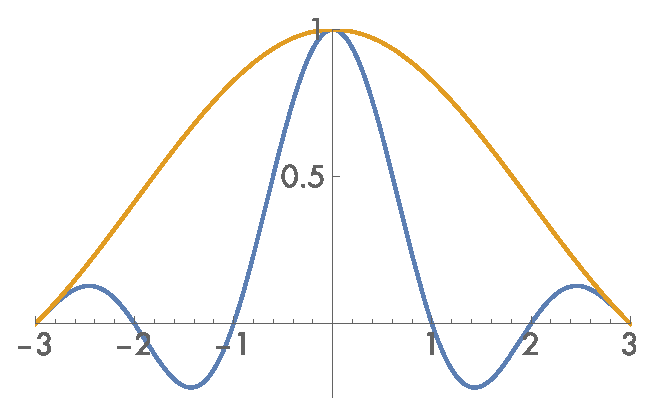
\includegraphics[width=0.49\linewidth]{chap07/sinc-and-window.eps}\label{fig:7.45.1}}\,
    \subfloat[]{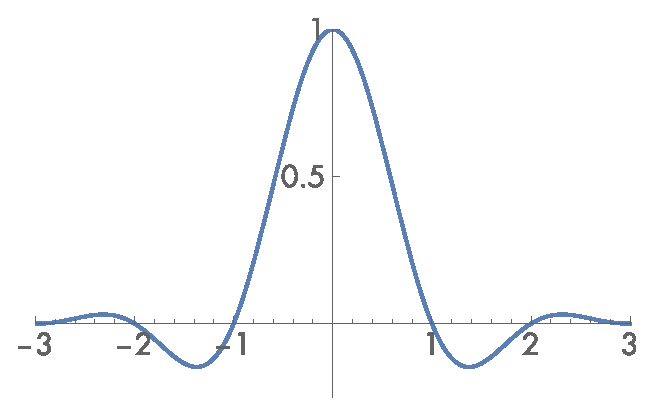
\includegraphics[width=0.49\linewidth]{chap07/sinc-times-window.eps}\label{fig:7.45.2}}
    \caption{sinc滤波器的图示。(a)三个周期后被截断了的sinc函数(蓝线)
        以及Lanczos窗函数(橙线)。(b)这两个函数的乘积,正如在\refvar{LanczosSincFilter}{}中的实现。}
    \label{fig:7.45}
\end{figure}

\reffig{7.46}为均匀1D样本展示了加窗的sinc重建结果。
因为加窗,重建的阶跃函数比用无限范围sinc函数重建的展现出小得多的振铃
(和\reffig{7.11}比较)。加窗的sinc滤波器在重建正弦函数时也做得极好,直到预混叠开始。
\begin{figure}[htbp]
    \centering
    \subfloat[]{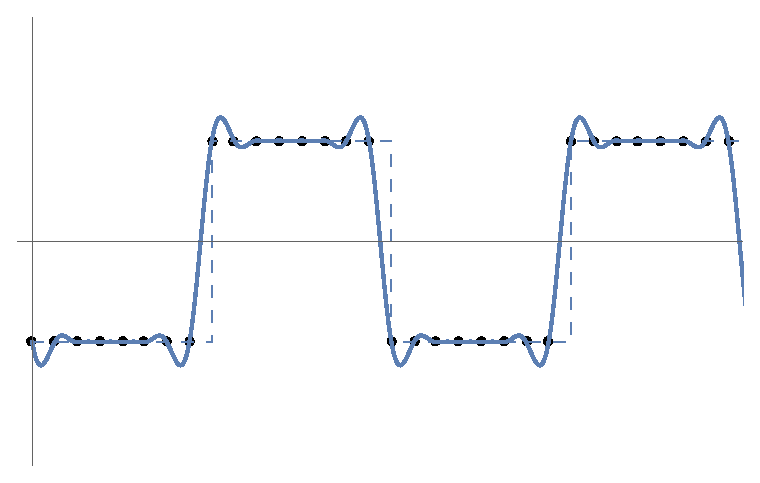
\includegraphics[width=0.49\linewidth]{chap07/sinc-recon-a.eps}\label{fig:7.46.1}}\,
    \subfloat[]{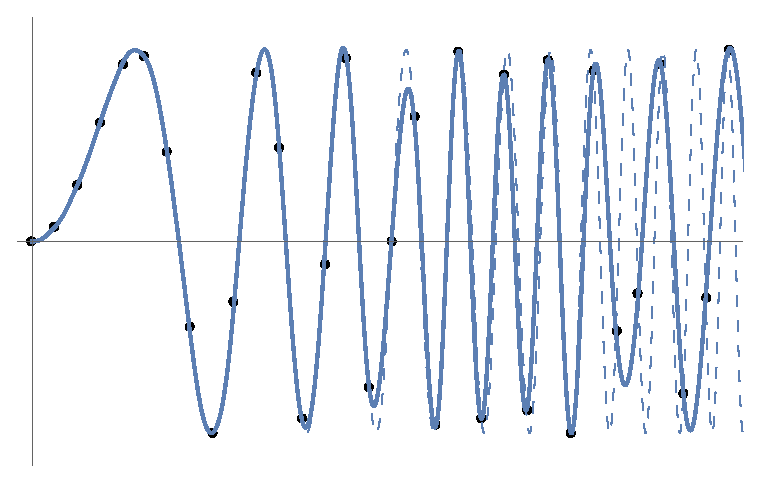
\includegraphics[width=0.49\linewidth]{chap07/sinc-recon-b.eps}}
    \caption{用加窗sinc滤波器重建示例函数的结果。这里$\tau=3$.
        (a)像无限sinc那样,对于阶跃函数它也遭受了振铃,尽管在加窗版本中的振铃要少得多。
        (b)然而滤波器对于正弦函数做得很好。}
    \label{fig:7.46}
\end{figure}

\begin{lstlisting}
`\initcode{Sinc Filter Declarations}{=}`
class `\initvar{LanczosSincFilter}{}` : public `\refvar{Filter}{}` {
public:
    `\refcode{LanczosSincFilter Public Methods}{}`
private:
    const `\refvar{Float}{}` `\initvar[LanczosSincFilter::tau]{tau}{}`;
};
\end{lstlisting}
\begin{lstlisting}
`\initcode{LanczosSincFilter Public Methods}{=}\initnext{LanczosSincFilterPublicMethods}`
`\refvar{LanczosSincFilter}{}`(const `\refvar{Vector2f}{}` &radius, `\refvar{Float}{}` tau)
    : `\refvar{Filter}{}`(radius), `\refvar[LanczosSincFilter::tau]{tau}{}`(tau) { }
\end{lstlisting}
\begin{lstlisting}
`\initcode{Sinc Filter Method Definitions}{=}`
`\refvar{Float}{}` `\refvar{LanczosSincFilter}{}`::`\initvar[LanczosSincFilter::Evaluate]{\refvar[Filter::Evaluate]{Evaluate}{}}{}`(const `\refvar{Point2f}{}` &p) const {
    return `\refvar{WindowedSinc}{}`(p.x, `\refvar[Filter::radius]{radius}{}`.x) * `\refvar{WindowedSinc}{}`(p.y, `\refvar[Filter::radius]{radius}{}`.y);
}
\end{lstlisting}

该实现计算sinc函数值然后乘以Lanczos窗函数值。
\begin{lstlisting}
`\refcode{LanczosSincFilter Public Methods}{+=}\lastnext{LanczosSincFilterPublicMethods}`
`\refvar{Float}{}` `\initvar{Sinc}{}`(`\refvar{Float}{}` x) const {
    x = std::abs(x);
    if (x < 1e-5)  return 1;
    return std::sin(`\refvar{Pi}{}` * x) / (`\refvar{Pi}{}` * x);
}
\end{lstlisting}
\begin{lstlisting}
`\refcode{LanczosSincFilter Public Methods}{+=}\lastcode{LanczosSincFilterPublicMethods}`
`\refvar{Float}{}` `\initvar{WindowedSinc}{}`(`\refvar{Float}{}` x, `\refvar{Float}{}` radius) const {
    x = std::abs(x);
    if (x > radius) return 0;
    `\refvar{Float}{}` lanczos = `\refvar{Sinc}{}`(x / `\refvar[LanczosSincFilter::tau]{tau}{}`);
    return `\refvar{Sinc}{}`(x) * lanczos;
}
\end{lstlisting}